% Created by tikzDevice version 0.12.6 on 2025-02-04 13:53:45
% !TEX encoding = UTF-8 Unicode
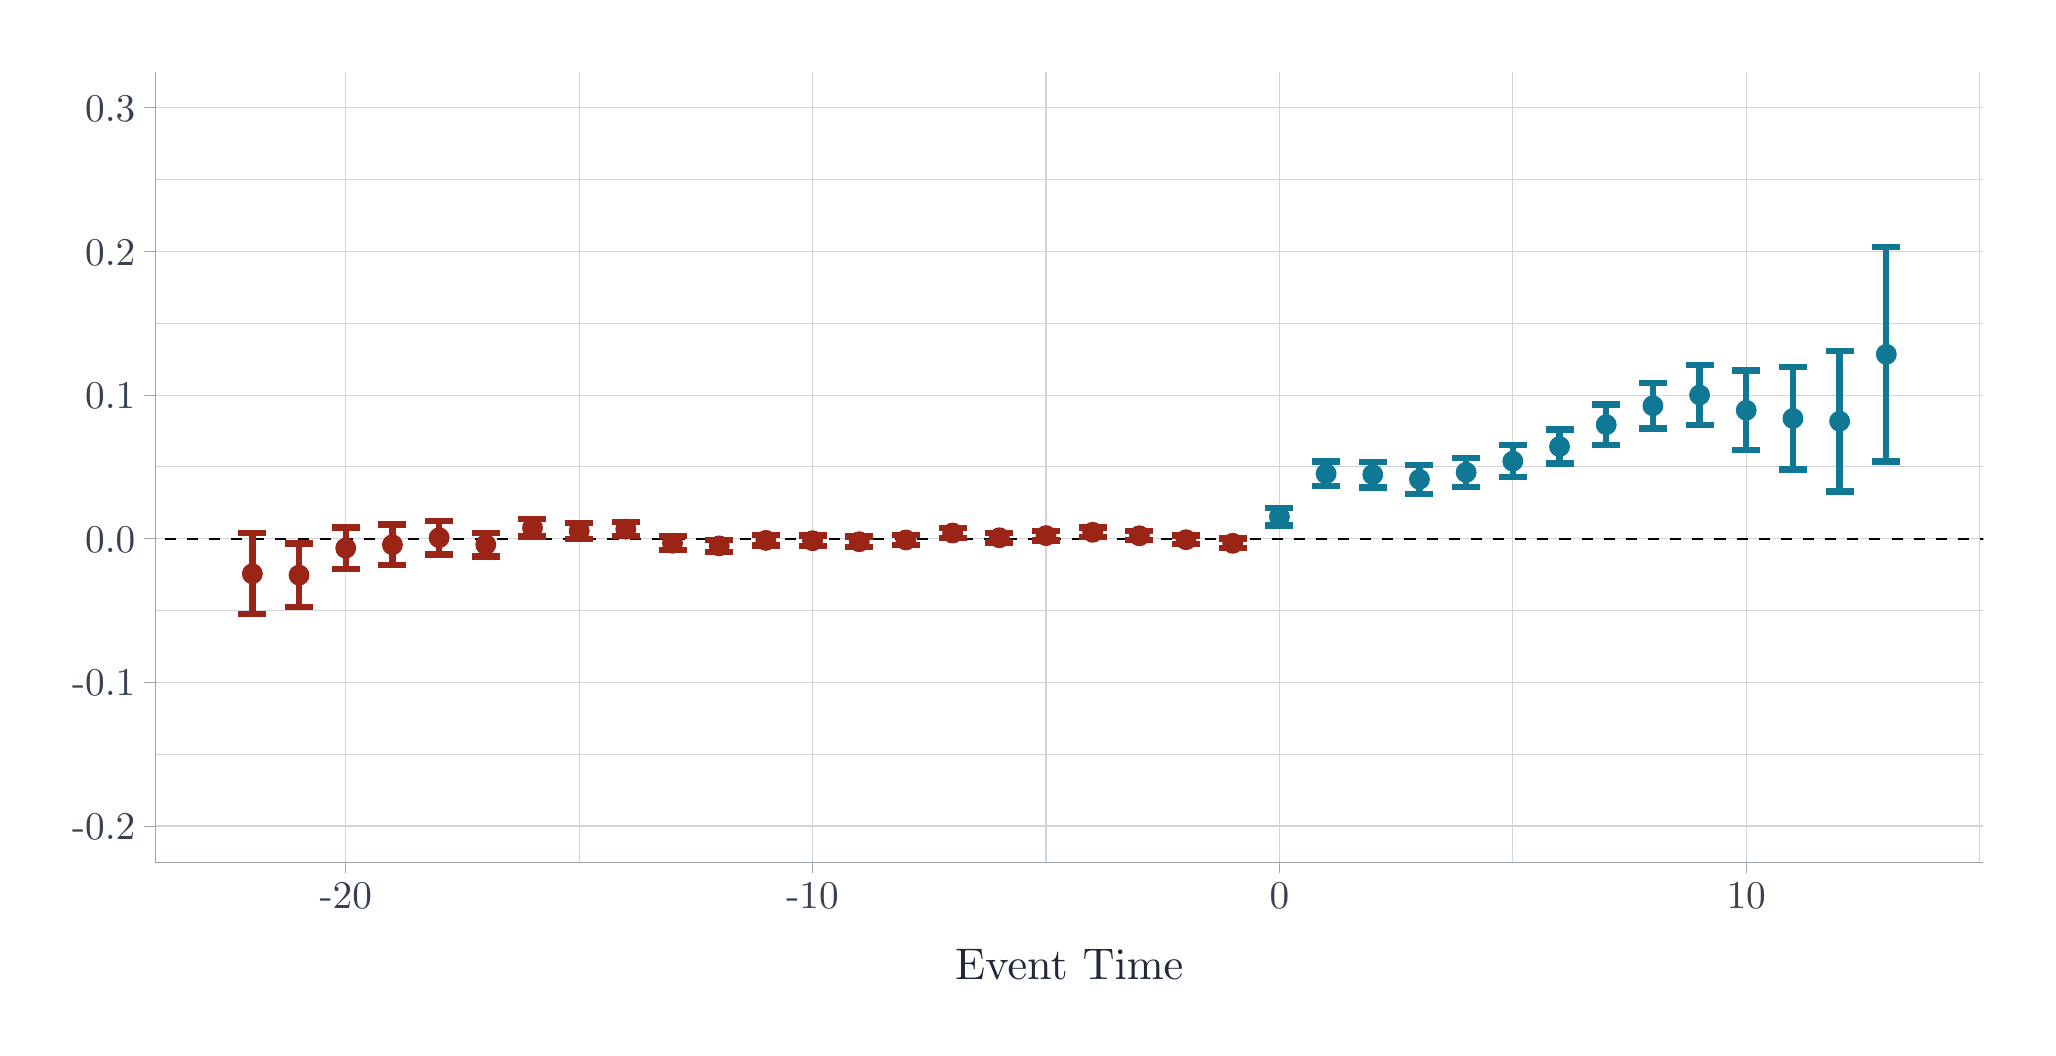
\begin{tikzpicture}[x=1pt,y=1pt]
\definecolor{fillColor}{RGB}{255,255,255}
\path[use as bounding box,fill=fillColor] (0,0) rectangle (722.70,361.35);
\begin{scope}
\path[clip] (  0.00,  0.00) rectangle (722.70,361.35);
\definecolor{drawColor}{RGB}{255,255,255}

\path[draw=drawColor,line width= 0.8pt,line join=round,line cap=round,fill=fillColor] (  0.00,  0.00) rectangle (722.70,361.35);
\end{scope}
\begin{scope}
\path[clip] ( 46.10, 59.89) rectangle (706.70,345.35);
\definecolor{drawColor}{RGB}{255,255,255}
\definecolor{fillColor}{RGB}{255,255,255}

\path[draw=drawColor,line width= 0.8pt,line join=round,line cap=round,fill=fillColor] ( 46.10, 59.89) rectangle (706.70,345.35);
\definecolor{drawColor}{RGB}{209,213,219}

\path[draw=drawColor,line width= 0.4pt,line join=round] ( 46.10, 98.81) --
	(706.70, 98.81);

\path[draw=drawColor,line width= 0.4pt,line join=round] ( 46.10,150.72) --
	(706.70,150.72);

\path[draw=drawColor,line width= 0.4pt,line join=round] ( 46.10,202.62) --
	(706.70,202.62);

\path[draw=drawColor,line width= 0.4pt,line join=round] ( 46.10,254.52) --
	(706.70,254.52);

\path[draw=drawColor,line width= 0.4pt,line join=round] ( 46.10,306.42) --
	(706.70,306.42);

\path[draw=drawColor,line width= 0.4pt,line join=round] (199.28, 59.89) --
	(199.28,345.35);

\path[draw=drawColor,line width= 0.4pt,line join=round] (367.97, 59.89) --
	(367.97,345.35);

\path[draw=drawColor,line width= 0.4pt,line join=round] (536.66, 59.89) --
	(536.66,345.35);

\path[draw=drawColor,line width= 0.4pt,line join=round] (705.35, 59.89) --
	(705.35,345.35);

\path[draw=drawColor,line width= 0.4pt,line join=round] ( 46.10, 72.86) --
	(706.70, 72.86);

\path[draw=drawColor,line width= 0.4pt,line join=round] ( 46.10,124.77) --
	(706.70,124.77);

\path[draw=drawColor,line width= 0.4pt,line join=round] ( 46.10,176.67) --
	(706.70,176.67);

\path[draw=drawColor,line width= 0.4pt,line join=round] ( 46.10,228.57) --
	(706.70,228.57);

\path[draw=drawColor,line width= 0.4pt,line join=round] ( 46.10,280.47) --
	(706.70,280.47);

\path[draw=drawColor,line width= 0.4pt,line join=round] ( 46.10,332.37) --
	(706.70,332.37);

\path[draw=drawColor,line width= 0.4pt,line join=round] (114.93, 59.89) --
	(114.93,345.35);

\path[draw=drawColor,line width= 0.4pt,line join=round] (283.62, 59.89) --
	(283.62,345.35);

\path[draw=drawColor,line width= 0.4pt,line join=round] (452.31, 59.89) --
	(452.31,345.35);

\path[draw=drawColor,line width= 0.4pt,line join=round] (621.00, 59.89) --
	(621.00,345.35);
\definecolor{drawColor}{RGB}{0,0,0}

\path[draw=drawColor,line width= 0.9pt,dash pattern=on 4pt off 4pt ,line join=round] (-614.49,176.67) -- (1367.30,176.67);
\definecolor{drawColor}{RGB}{154,36,21}
\definecolor{fillColor}{RGB}{154,36,21}

\path[draw=drawColor,line width= 0.4pt,line join=round,line cap=round,fill=fillColor] ( 81.19,164.02) circle (  3.57);

\path[draw=drawColor,line width= 0.4pt,line join=round,line cap=round,fill=fillColor] ( 98.06,163.53) circle (  3.57);

\path[draw=drawColor,line width= 0.4pt,line join=round,line cap=round,fill=fillColor] (114.93,173.28) circle (  3.57);

\path[draw=drawColor,line width= 0.4pt,line join=round,line cap=round,fill=fillColor] (131.80,174.48) circle (  3.57);

\path[draw=drawColor,line width= 0.4pt,line join=round,line cap=round,fill=fillColor] (148.67,177.05) circle (  3.57);

\path[draw=drawColor,line width= 0.4pt,line join=round,line cap=round,fill=fillColor] (165.54,174.53) circle (  3.57);

\path[draw=drawColor,line width= 0.4pt,line join=round,line cap=round,fill=fillColor] (182.41,180.62) circle (  3.57);

\path[draw=drawColor,line width= 0.4pt,line join=round,line cap=round,fill=fillColor] (199.28,179.48) circle (  3.57);

\path[draw=drawColor,line width= 0.4pt,line join=round,line cap=round,fill=fillColor] (216.15,180.14) circle (  3.57);

\path[draw=drawColor,line width= 0.4pt,line join=round,line cap=round,fill=fillColor] (233.01,175.05) circle (  3.57);

\path[draw=drawColor,line width= 0.4pt,line join=round,line cap=round,fill=fillColor] (249.88,174.09) circle (  3.57);

\path[draw=drawColor,line width= 0.4pt,line join=round,line cap=round,fill=fillColor] (266.75,176.07) circle (  3.57);

\path[draw=drawColor,line width= 0.4pt,line join=round,line cap=round,fill=fillColor] (283.62,175.96) circle (  3.57);

\path[draw=drawColor,line width= 0.4pt,line join=round,line cap=round,fill=fillColor] (300.49,175.59) circle (  3.57);

\path[draw=drawColor,line width= 0.4pt,line join=round,line cap=round,fill=fillColor] (317.36,176.23) circle (  3.57);

\path[draw=drawColor,line width= 0.4pt,line join=round,line cap=round,fill=fillColor] (334.23,178.73) circle (  3.57);

\path[draw=drawColor,line width= 0.4pt,line join=round,line cap=round,fill=fillColor] (351.10,177.02) circle (  3.57);

\path[draw=drawColor,line width= 0.4pt,line join=round,line cap=round,fill=fillColor] (367.97,177.80) circle (  3.57);

\path[draw=drawColor,line width= 0.4pt,line join=round,line cap=round,fill=fillColor] (384.84,179.00) circle (  3.57);

\path[draw=drawColor,line width= 0.4pt,line join=round,line cap=round,fill=fillColor] (401.71,177.74) circle (  3.57);

\path[draw=drawColor,line width= 0.4pt,line join=round,line cap=round,fill=fillColor] (418.58,176.32) circle (  3.57);

\path[draw=drawColor,line width= 0.4pt,line join=round,line cap=round,fill=fillColor] (435.44,175.02) circle (  3.57);
\definecolor{drawColor}{RGB}{16,120,149}
\definecolor{fillColor}{RGB}{16,120,149}

\path[draw=drawColor,line width= 0.4pt,line join=round,line cap=round,fill=fillColor] (452.31,184.63) circle (  3.57);

\path[draw=drawColor,line width= 0.4pt,line join=round,line cap=round,fill=fillColor] (469.18,200.18) circle (  3.57);

\path[draw=drawColor,line width= 0.4pt,line join=round,line cap=round,fill=fillColor] (486.05,199.85) circle (  3.57);

\path[draw=drawColor,line width= 0.4pt,line join=round,line cap=round,fill=fillColor] (502.92,198.14) circle (  3.57);

\path[draw=drawColor,line width= 0.4pt,line join=round,line cap=round,fill=fillColor] (519.79,200.66) circle (  3.57);

\path[draw=drawColor,line width= 0.4pt,line join=round,line cap=round,fill=fillColor] (536.66,204.70) circle (  3.57);

\path[draw=drawColor,line width= 0.4pt,line join=round,line cap=round,fill=fillColor] (553.53,209.99) circle (  3.57);

\path[draw=drawColor,line width= 0.4pt,line join=round,line cap=round,fill=fillColor] (570.40,217.88) circle (  3.57);

\path[draw=drawColor,line width= 0.4pt,line join=round,line cap=round,fill=fillColor] (587.27,224.72) circle (  3.57);

\path[draw=drawColor,line width= 0.4pt,line join=round,line cap=round,fill=fillColor] (604.14,228.62) circle (  3.57);

\path[draw=drawColor,line width= 0.4pt,line join=round,line cap=round,fill=fillColor] (621.00,223.10) circle (  3.57);

\path[draw=drawColor,line width= 0.4pt,line join=round,line cap=round,fill=fillColor] (637.87,220.14) circle (  3.57);

\path[draw=drawColor,line width= 0.4pt,line join=round,line cap=round,fill=fillColor] (654.74,219.15) circle (  3.57);

\path[draw=drawColor,line width= 0.4pt,line join=round,line cap=round,fill=fillColor] (671.61,243.31) circle (  3.57);
\definecolor{drawColor}{RGB}{154,36,21}

\path[draw=drawColor,line width= 2.3pt,line join=round] ( 76.13,178.65) --
	( 86.25,178.65);

\path[draw=drawColor,line width= 2.3pt,line join=round] ( 81.19,178.65) --
	( 81.19,149.39);

\path[draw=drawColor,line width= 2.3pt,line join=round] ( 76.13,149.39) --
	( 86.25,149.39);

\path[draw=drawColor,line width= 2.3pt,line join=round] ( 93.00,174.99) --
	(103.12,174.99);

\path[draw=drawColor,line width= 2.3pt,line join=round] ( 98.06,174.99) --
	( 98.06,152.07);

\path[draw=drawColor,line width= 2.3pt,line join=round] ( 93.00,152.07) --
	(103.12,152.07);

\path[draw=drawColor,line width= 2.3pt,line join=round] (109.87,180.78) --
	(119.99,180.78);

\path[draw=drawColor,line width= 2.3pt,line join=round] (114.93,180.78) --
	(114.93,165.77);

\path[draw=drawColor,line width= 2.3pt,line join=round] (109.87,165.77) --
	(119.99,165.77);

\path[draw=drawColor,line width= 2.3pt,line join=round] (126.74,181.88) --
	(136.86,181.88);

\path[draw=drawColor,line width= 2.3pt,line join=round] (131.80,181.88) --
	(131.80,167.09);

\path[draw=drawColor,line width= 2.3pt,line join=round] (126.74,167.09) --
	(136.86,167.09);

\path[draw=drawColor,line width= 2.3pt,line join=round] (143.61,183.12) --
	(153.73,183.12);

\path[draw=drawColor,line width= 2.3pt,line join=round] (148.67,183.12) --
	(148.67,170.98);

\path[draw=drawColor,line width= 2.3pt,line join=round] (143.61,170.98) --
	(153.73,170.98);

\path[draw=drawColor,line width= 2.3pt,line join=round] (160.48,178.77) --
	(170.60,178.77);

\path[draw=drawColor,line width= 2.3pt,line join=round] (165.54,178.77) --
	(165.54,170.29);

\path[draw=drawColor,line width= 2.3pt,line join=round] (160.48,170.29) --
	(170.60,170.29);

\path[draw=drawColor,line width= 2.3pt,line join=round] (177.35,183.80) --
	(187.47,183.80);

\path[draw=drawColor,line width= 2.3pt,line join=round] (182.41,183.80) --
	(182.41,177.45);

\path[draw=drawColor,line width= 2.3pt,line join=round] (177.35,177.45) --
	(187.47,177.45);

\path[draw=drawColor,line width= 2.3pt,line join=round] (194.22,182.29) --
	(204.34,182.29);

\path[draw=drawColor,line width= 2.3pt,line join=round] (199.28,182.29) --
	(199.28,176.68);

\path[draw=drawColor,line width= 2.3pt,line join=round] (194.22,176.68) --
	(204.34,176.68);

\path[draw=drawColor,line width= 2.3pt,line join=round] (211.08,182.73) --
	(221.21,182.73);

\path[draw=drawColor,line width= 2.3pt,line join=round] (216.15,182.73) --
	(216.15,177.55);

\path[draw=drawColor,line width= 2.3pt,line join=round] (211.08,177.55) --
	(221.21,177.55);

\path[draw=drawColor,line width= 2.3pt,line join=round] (227.95,177.62) --
	(238.08,177.62);

\path[draw=drawColor,line width= 2.3pt,line join=round] (233.01,177.62) --
	(233.01,172.49);

\path[draw=drawColor,line width= 2.3pt,line join=round] (227.95,172.49) --
	(238.08,172.49);

\path[draw=drawColor,line width= 2.3pt,line join=round] (244.82,176.27) --
	(254.94,176.27);

\path[draw=drawColor,line width= 2.3pt,line join=round] (249.88,176.27) --
	(249.88,171.91);

\path[draw=drawColor,line width= 2.3pt,line join=round] (244.82,171.91) --
	(254.94,171.91);

\path[draw=drawColor,line width= 2.3pt,line join=round] (261.69,177.95) --
	(271.81,177.95);

\path[draw=drawColor,line width= 2.3pt,line join=round] (266.75,177.95) --
	(266.75,174.20);

\path[draw=drawColor,line width= 2.3pt,line join=round] (261.69,174.20) --
	(271.81,174.20);

\path[draw=drawColor,line width= 2.3pt,line join=round] (278.56,177.78) --
	(288.68,177.78);

\path[draw=drawColor,line width= 2.3pt,line join=round] (283.62,177.78) --
	(283.62,174.14);

\path[draw=drawColor,line width= 2.3pt,line join=round] (278.56,174.14) --
	(288.68,174.14);

\path[draw=drawColor,line width= 2.3pt,line join=round] (295.43,177.48) --
	(305.55,177.48);

\path[draw=drawColor,line width= 2.3pt,line join=round] (300.49,177.48) --
	(300.49,173.71);

\path[draw=drawColor,line width= 2.3pt,line join=round] (295.43,173.71) --
	(305.55,173.71);

\path[draw=drawColor,line width= 2.3pt,line join=round] (312.30,177.97) --
	(322.42,177.97);

\path[draw=drawColor,line width= 2.3pt,line join=round] (317.36,177.97) --
	(317.36,174.49);

\path[draw=drawColor,line width= 2.3pt,line join=round] (312.30,174.49) --
	(322.42,174.49);

\path[draw=drawColor,line width= 2.3pt,line join=round] (329.17,180.47) --
	(339.29,180.47);

\path[draw=drawColor,line width= 2.3pt,line join=round] (334.23,180.47) --
	(334.23,176.99);

\path[draw=drawColor,line width= 2.3pt,line join=round] (329.17,176.99) --
	(339.29,176.99);

\path[draw=drawColor,line width= 2.3pt,line join=round] (346.04,178.77) --
	(356.16,178.77);

\path[draw=drawColor,line width= 2.3pt,line join=round] (351.10,178.77) --
	(351.10,175.26);

\path[draw=drawColor,line width= 2.3pt,line join=round] (346.04,175.26) --
	(356.16,175.26);

\path[draw=drawColor,line width= 2.3pt,line join=round] (362.91,179.57) --
	(373.03,179.57);

\path[draw=drawColor,line width= 2.3pt,line join=round] (367.97,179.57) --
	(367.97,176.03);

\path[draw=drawColor,line width= 2.3pt,line join=round] (362.91,176.03) --
	(373.03,176.03);

\path[draw=drawColor,line width= 2.3pt,line join=round] (379.78,180.74) --
	(389.90,180.74);

\path[draw=drawColor,line width= 2.3pt,line join=round] (384.84,180.74) --
	(384.84,177.25);

\path[draw=drawColor,line width= 2.3pt,line join=round] (379.78,177.25) --
	(389.90,177.25);

\path[draw=drawColor,line width= 2.3pt,line join=round] (396.65,179.36) --
	(406.77,179.36);

\path[draw=drawColor,line width= 2.3pt,line join=round] (401.71,179.36) --
	(401.71,176.13);

\path[draw=drawColor,line width= 2.3pt,line join=round] (396.65,176.13) --
	(406.77,176.13);

\path[draw=drawColor,line width= 2.3pt,line join=round] (413.51,177.78) --
	(423.64,177.78);

\path[draw=drawColor,line width= 2.3pt,line join=round] (418.58,177.78) --
	(418.58,174.87);

\path[draw=drawColor,line width= 2.3pt,line join=round] (413.51,174.87) --
	(423.64,174.87);

\path[draw=drawColor,line width= 2.3pt,line join=round] (430.38,176.74) --
	(440.50,176.74);

\path[draw=drawColor,line width= 2.3pt,line join=round] (435.44,176.74) --
	(435.44,173.30);

\path[draw=drawColor,line width= 2.3pt,line join=round] (430.38,173.30) --
	(440.50,173.30);
\definecolor{drawColor}{RGB}{16,120,149}

\path[draw=drawColor,line width= 2.3pt,line join=round] (447.25,187.87) --
	(457.37,187.87);

\path[draw=drawColor,line width= 2.3pt,line join=round] (452.31,187.87) --
	(452.31,181.40);

\path[draw=drawColor,line width= 2.3pt,line join=round] (447.25,181.40) --
	(457.37,181.40);

\path[draw=drawColor,line width= 2.3pt,line join=round] (464.12,204.53) --
	(474.24,204.53);

\path[draw=drawColor,line width= 2.3pt,line join=round] (469.18,204.53) --
	(469.18,195.84);

\path[draw=drawColor,line width= 2.3pt,line join=round] (464.12,195.84) --
	(474.24,195.84);

\path[draw=drawColor,line width= 2.3pt,line join=round] (480.99,204.49) --
	(491.11,204.49);

\path[draw=drawColor,line width= 2.3pt,line join=round] (486.05,204.49) --
	(486.05,195.22);

\path[draw=drawColor,line width= 2.3pt,line join=round] (480.99,195.22) --
	(491.11,195.22);

\path[draw=drawColor,line width= 2.3pt,line join=round] (497.86,203.36) --
	(507.98,203.36);

\path[draw=drawColor,line width= 2.3pt,line join=round] (502.92,203.36) --
	(502.92,192.92);

\path[draw=drawColor,line width= 2.3pt,line join=round] (497.86,192.92) --
	(507.98,192.92);

\path[draw=drawColor,line width= 2.3pt,line join=round] (514.73,205.92) --
	(524.85,205.92);

\path[draw=drawColor,line width= 2.3pt,line join=round] (519.79,205.92) --
	(519.79,195.40);

\path[draw=drawColor,line width= 2.3pt,line join=round] (514.73,195.40) --
	(524.85,195.40);

\path[draw=drawColor,line width= 2.3pt,line join=round] (531.60,210.49) --
	(541.72,210.49);

\path[draw=drawColor,line width= 2.3pt,line join=round] (536.66,210.49) --
	(536.66,198.91);

\path[draw=drawColor,line width= 2.3pt,line join=round] (531.60,198.91) --
	(541.72,198.91);

\path[draw=drawColor,line width= 2.3pt,line join=round] (548.47,216.11) --
	(558.59,216.11);

\path[draw=drawColor,line width= 2.3pt,line join=round] (553.53,216.11) --
	(553.53,203.87);

\path[draw=drawColor,line width= 2.3pt,line join=round] (548.47,203.87) --
	(558.59,203.87);

\path[draw=drawColor,line width= 2.3pt,line join=round] (565.34,225.12) --
	(575.46,225.12);

\path[draw=drawColor,line width= 2.3pt,line join=round] (570.40,225.12) --
	(570.40,210.64);

\path[draw=drawColor,line width= 2.3pt,line join=round] (565.34,210.64) --
	(575.46,210.64);

\path[draw=drawColor,line width= 2.3pt,line join=round] (582.21,232.99) --
	(592.33,232.99);

\path[draw=drawColor,line width= 2.3pt,line join=round] (587.27,232.99) --
	(587.27,216.45);

\path[draw=drawColor,line width= 2.3pt,line join=round] (582.21,216.45) --
	(592.33,216.45);

\path[draw=drawColor,line width= 2.3pt,line join=round] (599.07,239.39) --
	(609.20,239.39);

\path[draw=drawColor,line width= 2.3pt,line join=round] (604.14,239.39) --
	(604.14,217.85);

\path[draw=drawColor,line width= 2.3pt,line join=round] (599.07,217.85) --
	(609.20,217.85);

\path[draw=drawColor,line width= 2.3pt,line join=round] (615.94,237.51) --
	(626.07,237.51);

\path[draw=drawColor,line width= 2.3pt,line join=round] (621.00,237.51) --
	(621.00,208.69);

\path[draw=drawColor,line width= 2.3pt,line join=round] (615.94,208.69) --
	(626.07,208.69);

\path[draw=drawColor,line width= 2.3pt,line join=round] (632.81,238.65) --
	(642.93,238.65);

\path[draw=drawColor,line width= 2.3pt,line join=round] (637.87,238.65) --
	(637.87,201.63);

\path[draw=drawColor,line width= 2.3pt,line join=round] (632.81,201.63) --
	(642.93,201.63);

\path[draw=drawColor,line width= 2.3pt,line join=round] (649.68,244.59) --
	(659.80,244.59);

\path[draw=drawColor,line width= 2.3pt,line join=round] (654.74,244.59) --
	(654.74,193.71);

\path[draw=drawColor,line width= 2.3pt,line join=round] (649.68,193.71) --
	(659.80,193.71);

\path[draw=drawColor,line width= 2.3pt,line join=round] (666.55,281.98) --
	(676.67,281.98);

\path[draw=drawColor,line width= 2.3pt,line join=round] (671.61,281.98) --
	(671.61,204.64);

\path[draw=drawColor,line width= 2.3pt,line join=round] (666.55,204.64) --
	(676.67,204.64);
\end{scope}
\begin{scope}
\path[clip] (  0.00,  0.00) rectangle (722.70,361.35);
\definecolor{drawColor}{RGB}{156,163,175}

\path[draw=drawColor,line width= 0.3pt,line join=round] ( 46.10, 59.89) --
	( 46.10,345.35);
\end{scope}
\begin{scope}
\path[clip] (  0.00,  0.00) rectangle (722.70,361.35);
\definecolor{drawColor}{RGB}{55,65,81}

\node[text=drawColor,anchor=base east,inner sep=0pt, outer sep=0pt, scale=  1.42] at ( 38.90, 67.97) {-0.2};

\node[text=drawColor,anchor=base east,inner sep=0pt, outer sep=0pt, scale=  1.42] at ( 38.90,119.87) {-0.1};

\node[text=drawColor,anchor=base east,inner sep=0pt, outer sep=0pt, scale=  1.42] at ( 38.90,171.77) {0.0};

\node[text=drawColor,anchor=base east,inner sep=0pt, outer sep=0pt, scale=  1.42] at ( 38.90,223.67) {0.1};

\node[text=drawColor,anchor=base east,inner sep=0pt, outer sep=0pt, scale=  1.42] at ( 38.90,275.58) {0.2};

\node[text=drawColor,anchor=base east,inner sep=0pt, outer sep=0pt, scale=  1.42] at ( 38.90,327.48) {0.3};
\end{scope}
\begin{scope}
\path[clip] (  0.00,  0.00) rectangle (722.70,361.35);
\definecolor{drawColor}{RGB}{156,163,175}

\path[draw=drawColor,line width= 0.3pt,line join=round] ( 42.10, 72.86) --
	( 46.10, 72.86);

\path[draw=drawColor,line width= 0.3pt,line join=round] ( 42.10,124.77) --
	( 46.10,124.77);

\path[draw=drawColor,line width= 0.3pt,line join=round] ( 42.10,176.67) --
	( 46.10,176.67);

\path[draw=drawColor,line width= 0.3pt,line join=round] ( 42.10,228.57) --
	( 46.10,228.57);

\path[draw=drawColor,line width= 0.3pt,line join=round] ( 42.10,280.47) --
	( 46.10,280.47);

\path[draw=drawColor,line width= 0.3pt,line join=round] ( 42.10,332.37) --
	( 46.10,332.37);
\end{scope}
\begin{scope}
\path[clip] (  0.00,  0.00) rectangle (722.70,361.35);
\definecolor{drawColor}{RGB}{156,163,175}

\path[draw=drawColor,line width= 0.3pt,line join=round] ( 46.10, 59.89) --
	(706.70, 59.89);
\end{scope}
\begin{scope}
\path[clip] (  0.00,  0.00) rectangle (722.70,361.35);
\definecolor{drawColor}{RGB}{156,163,175}

\path[draw=drawColor,line width= 0.3pt,line join=round] (114.93, 55.89) --
	(114.93, 59.89);

\path[draw=drawColor,line width= 0.3pt,line join=round] (283.62, 55.89) --
	(283.62, 59.89);

\path[draw=drawColor,line width= 0.3pt,line join=round] (452.31, 55.89) --
	(452.31, 59.89);

\path[draw=drawColor,line width= 0.3pt,line join=round] (621.00, 55.89) --
	(621.00, 59.89);
\end{scope}
\begin{scope}
\path[clip] (  0.00,  0.00) rectangle (722.70,361.35);
\definecolor{drawColor}{RGB}{55,65,81}

\node[text=drawColor,anchor=base,inner sep=0pt, outer sep=0pt, scale=  1.42] at (114.93, 42.89) {-20};

\node[text=drawColor,anchor=base,inner sep=0pt, outer sep=0pt, scale=  1.42] at (283.62, 42.89) {-10};

\node[text=drawColor,anchor=base,inner sep=0pt, outer sep=0pt, scale=  1.42] at (452.31, 42.89) {0};

\node[text=drawColor,anchor=base,inner sep=0pt, outer sep=0pt, scale=  1.42] at (621.00, 42.89) {10};
\end{scope}
\begin{scope}
\path[clip] (  0.00,  0.00) rectangle (722.70,361.35);
\definecolor{drawColor}{RGB}{31,41,55}

\node[text=drawColor,anchor=base,inner sep=0pt, outer sep=0pt, scale=  1.60] at (376.40, 17.56) {Event Time};
\end{scope}
\end{tikzpicture}
